\chapter{MIT bag model}

Smoothly introduce concepts in intro and some other concepts (like bag constant and strange matter hypothesis)

A classic

Treat two and three flavor versions together: they are very similar.
Therefore write $(s)$.

Constant masses $m_u = \ldots$ etc.

QCD Lagrangian when neglecting gluons completely:
\begin{equation}
	\lagr = \bar{q} (i \slashed\partial + \mu \gamma^0 - m) q
	      = \sum_{c=1}^{N_c} \sum_{f=\{u,d,(s)\}} \bar{q}_{f,c} (i \slashed\partial + \mu_f \gamma^0 - m_f) q_{f,c}
\label{eq:mit:lagrangian}
\end{equation}

\section{Partition function, grand potential and equation of state}

With the Euclidean version of the Lagrangian density \eqref{eq:mit:lagrangian},
the partition function \eqref{eq:master_intro:partition_function} reads
\begin{equation}
	Z(V, T, \mu_i) = \prod_{c=1}^{N_c} \prod_{f=\{u,d,(s)\}} \oint_- \pathintdif \bar{q}_{f,c} \oint_- \pathintdif q_{f,c} \exp \bigg\{ \int_0^\beta \dif \tau \int_V \dif^3 x \lagr_E [q_{f,c},\bar{q}_{f,c}] \bigg\} .
\end{equation}
It decouples into a product of path integrals \eqref{eq:tft:dirac_partition_function_first} that we encountered back in \cref{chap:tft}.
There we simplified these path integrals to the form \eqref{eq:tft:dirac_partition_function} for arbitrary temperature.
Then we neglected the vacuum contribution from the first term and calculated it explicitly in the zero-temperature approximation,
arriving at the pressure \eqref{eq:nstars:pressure_zeroT} that is related to the grand potential density \eqref{eq:master_intro:grand_potential} by a simple sign flip.
Adding a background of free electrons and reinstating the Fermi momenta $p_f = \sqrt{\mu_f^2-m_f^2}$ for each particle,
we can then write the grand potential density as
\begin{equation}
	\Omega(\mu_u,\mu_d,\mu_s,\mu_e) = -\smashoperator{\sum_{\vphantom{\big|} f=\{3u,3d,(3s),e\}}} \frac{1}{24 \pi^2} \left[ \left( 2 \mu_f^2 - 5 m_f^2 \right) \mu_f \sqrt{\mu_f^2 - m_f^2} + 3 m_f^4 \asinh \left( \sqrt{\frac{\mu_{\smash{f}}^2}{m_f^2}-1} \right) \right] .
\label{eq:mit:grand_potential}
\end{equation}
Our notation below the flavor sum means that the quark terms are multiplied by $N_c=3$,
but the electron contribution is not.
The corresponding quark and electron densities \eqref{eq:master_intro:densities} are
\begin{equation}
	n_f = -\pdv{\Omega}{\mu_f} = \frac{N_c}{3 \pi^2} \Big( \mu_f^2 - m_f^2 \Big)^{\frac32}
	\text{ for $f \in \{u,d,(s)\}$}
	\quad \text{and} \quad
	n_e = -\pdv{\Omega}{\mu_e} = \frac{  1}{3 \pi^2} \Big( \mu_e^2 - m_e^2 \Big)^{\frac32},
\label{eq:mit:particle_densities}%
\end{equation}
and the pressure \eqref{eq:master_intro:pressure} and energy density \eqref{eq:master_intro:energy_density} follow.

We now see explicitly that the grand potential and hence the pressure and energy density are functions of the four chemical potentials $\mu_u$, $\mu_d$, $\mu_s$ and $\mu_e$.
As explained in \cref{sec:master_intro:tft},
we reduce them to only one independent chemical potential with the three constraints \eqref{eq:lsm:chemical_equilibrium} and \eqref{eq:lsm:charge_neutrality} --
and take this to be the quark chemical potential $\mu_Q$ defined in equation \eqref{eq:master_intro:chemical_potentials_transformed}.
With the densities \eqref{eq:mit:particle_densities} and for a given value of $\mu_Q$,
we must then find the electron chemical potential $\mu_e$ that solves
\TODO{create and refer to table with quark properties: name, electric charges, two masses}
\begin{equation}
	2 \Big[\mu_u^2-m_u^2\Big]^\frac32
	- \Big[(\mu_u+\mu_e)^2-m_d^2\Big]^\frac32 
	- \Big[(\mu_u+\mu_e)^2-m_s^2\Big]^\frac32 
	- \Big[\mu_e^2-m_e^2\Big]^\frac32 = 0,
\label{eq:mit:charge_neutrality_explicit}
\end{equation}
after which the two remaining chemical potentials are given by the chemical equilibrium constraint \eqref{eq:lsm:chemical_equilibrium}. 
Elimination of the three chemical potentials yields two functions $P(\mu_u)$ and $\epsilon(\mu_u)$,
and the former can finally be inverted to yield the equation of state $\epsilon(P)$.
Using the program in \TODO{ref appendix},
we obtain the chemical potentials, densities and equation of state shown in \cref{fig:mit:eos}.

\begin{figure}
\centering
\tikzsetnextfilename{mit-eos}
\begin{tikzpicture}
\tikzset{declare function={
	muQ(\muu,\mud)=(\muu+\mud)/2;
	muu(\muQ)=2/(1+2^(1/3))*\muQ;
	mud(\muQ)=2/(1+2^(-1/3))*\muQ;
	mue(\muQ)=2*(2^(1/3)-1)/(2^(1/3)+1)*\muQ;
	nq(\mu)=3/(3*pi^2)*(\mu)^3;
	ne(\mu)=1/(3*pi^2)*(\mu)^3;
	nconv=1.29619e-7;
}};
\begin{groupplot}[
	group style={group size={1 by 3}, vertical sep=2.0cm},
	width=13cm, height=7cm,
	extra tick style={grid=major, grid style={dashed}},
	minor tick num=9,
]
\nextgroupplot[
	xlabel={$\mu_Q \, / \, \si{\mega\electronvolt}$}, ylabel={$\mu_i \, / \, \si{\mega\electronvolt}$},
	%xmin=0, xmax=600, ymax=500, xtick distance=100, ytick distance=100, minor x tick num=9,
	xmin=0, xmax=1000, xtick distance=100, minor x tick num=9,
	ymin=0, ymax=1000, ytick distance=100, 
	%ymax=600, 
	title={\subcaption{\label{fig:mit:eos-parametrization}Parametrization of solutions}},
	legend cell align=right, legend pos=north west,
];
% fake legend
\addplot+ [black, solid, opacity=0.3] {-100}; \addlegendentry{$N_f=2$};
\addplot+ [black, solid, opacity=0.8] {-100}; \addlegendentry{$N_f=3$};
\addplot+ [red, solid, opacity=1.0] {-100}; \addlegendentry{$i=u$};
\addplot+ [darkgreen, solid, opacity=1.0] {-100}; \addlegendentry{$i=d$};
\addplot+ [purple, solid, opacity=1.0] {-100}; \addlegendentry{$i=s$};
\addplot+ [blue, solid, opacity=1.0] {-100}; \addlegendentry{$i=e$};

% 2-flavor
\addplot+ [red,       solid,  opacity=0.3] table [x expr={muQ(\thisrow{muu},\thisrow{mud})}, y=muu] {../code/data/MIT2F/eos_sigma_800.dat};
\addplot+ [darkgreen, solid,  opacity=0.3] table [x expr={muQ(\thisrow{muu},\thisrow{mud})}, y=mud] {../code/data/MIT2F/eos_sigma_800.dat};
\addplot+ [blue,      solid,  opacity=0.3] table [x expr={muQ(\thisrow{muu},\thisrow{mud})}, y=mue] {../code/data/MIT2F/eos_sigma_800.dat};

% 3-flavor
\addplot+ [red,       solid,  opacity=0.8] table [x expr={muQ(\thisrow{muu},\thisrow{mud})}, y=muu] {../code/data/MIT3F/eos_sigma_800.dat};
\addplot+ [darkgreen, solid,  opacity=0.8] table [x expr={muQ(\thisrow{muu},\thisrow{mud})}, y=mud] {../code/data/MIT3F/eos_sigma_800.dat};
\addplot+ [purple,    dashed, opacity=0.8] table [x expr={muQ(\thisrow{muu},\thisrow{mud})}, y=mus] {../code/data/MIT3F/eos_sigma_800.dat};
\addplot+ [blue,      solid,  opacity=0.8] table [x expr={muQ(\thisrow{muu},\thisrow{mud})}, y=mue] {../code/data/MIT3F/eos_sigma_800.dat};

\nextgroupplot[
	xlabel={$\mu_Q \, / \, \si{\mega\electronvolt}$}, ylabel={$n_i \, / \, (1/\si{\femto\meter\cubed})$},
	xmin=0, xmax=1000, xtick distance=100, minor x tick num=9,
	ymin=-0.2, ymax=10.0, ytick distance=1.0, minor y tick num=4, restrict y to domain=-10:10,
	title={\subcaption{\label{fig:mit:eos-density}Particle number densities}},
	legend cell align=right, legend pos=north west,
];
% fake legend
\addplot+ [black, solid, opacity=0.3] {-10}; \addlegendentry{$N_f=2$};
\addplot+ [black, solid, opacity=0.8] {-10}; \addlegendentry{$N_f=3$};
\addplot+ [red, solid, opacity=1.0] {-10}; \addlegendentry{$i=u$};
\addplot+ [darkgreen, solid, opacity=1.0] {-10}; \addlegendentry{$i=d$};
\addplot+ [purple, solid, opacity=1.0] {-10}; \addlegendentry{$i=s$};
\addplot+ [blue, solid, opacity=1.0] {-10}; \addlegendentry{$i=e$};

% 2-flavor
\addplot+ [red,       solid, opacity=0.3] table [x expr={muQ(\thisrow{muu},\thisrow{mud})}, y=nu] {../code/data/MIT2F/eos_sigma_800.dat};
\addplot+ [darkgreen, solid, opacity=0.3] table [x expr={muQ(\thisrow{muu},\thisrow{mud})}, y=nd] {../code/data/MIT2F/eos_sigma_800.dat};
\addplot+ [blue,      solid, opacity=0.3] table [x expr={muQ(\thisrow{muu},\thisrow{mud})}, y=ne] {../code/data/MIT2F/eos_sigma_800.dat};

% 3-flavor
\addplot+ [red,       solid, opacity=0.8] table [x expr={muQ(\thisrow{muu},\thisrow{mud})}, y=nu] {../code/data/MIT3F/eos_sigma_800.dat};
\addplot+ [darkgreen, solid, opacity=0.8] table [x expr={muQ(\thisrow{muu},\thisrow{mud})}, y=nd] {../code/data/MIT3F/eos_sigma_800.dat};
\addplot+ [purple,    solid, opacity=0.8] table [x expr={muQ(\thisrow{muu},\thisrow{mud})}, y=ns] {../code/data/MIT3F/eos_sigma_800.dat};
\addplot+ [blue,      solid, opacity=0.8] table [x expr={muQ(\thisrow{muu},\thisrow{mud})}, y=ne] {../code/data/MIT3F/eos_sigma_800.dat};

\nextgroupplot[
	xlabel={$P        \, / \, (\si{\giga\electronvolt\per\femto\meter\cubed})$},
	ylabel={$\epsilon \, / \, (\si{\giga\electronvolt\per\femto\meter\cubed})$},
	xmin=0, xmax=0.30, ymin=0, ymax=1.0, xtick distance=0.10, minor x tick num=9, ytick distance=0.5, minor y tick num=4, restrict y to domain=-1:+1,
	title={\subcaption{\label{fig:mit:eos-eos}Equation of state}},
	legend cell align=left, legend pos=north west,
];
\addplot+ [black, solid, opacity=0.3] table [x=P,y=epsilon] {../code/data/MIT2F/eos_sigma_800.dat}; \addlegendentry{$N_f=2$};
\addplot+ [black, solid, opacity=0.8] table [x=P,y=epsilon] {../code/data/MIT3F/eos_sigma_800.dat}; \addlegendentry{$N_f=3$};
\end{groupplot}
\end{tikzpicture}
\caption{\label{fig:mit:eos}%
Properties of electrically charge neutral two-flavor (weak lines) and three-flavor (strong lines) MIT bag model quark matter in $\beta$-equilibrium parametrized by the common quark chemical potential $\mu_Q = (\mu_u+\mu_d)/2$.
Upper panel \subref{fig:mit:eos-parametrization} shows the relations between chemical potentials due to the constraints \eqref{eq:lsm:chemical_equilibrium} and \eqref{eq:lsm:charge_neutrality},
middle panel \subref{fig:mit:eos-density} the corresponding particle number densities \eqref{eq:mit:particle_densities} and
lower panel \subref{fig:mit:eos-eos} the resulting equation of state.
}
\end{figure}

\subsubsection{Ultra-relativistic limit}

Note that the electron density is very small, but nonzero,
and that the chemical potentials and equation of state seems to converge to a simple linear form in the ultra-relativistic limit $\mu_i \gg m_i$.
In fact, we can find analytical expressions for the chemical potentials, densities and equation of state in the limit $m_i \rightarrow 0$.
The grand potential \eqref{eq:mit:grand_potential} then reduces to
\begin{equation}
	\Omega(\mu_u, \mu_d, \mu_e) = -\frac{N_c \mu_u^4}{12 \pi^2} - \frac{N_c \mu_d^4}{12 \pi^2} - \frac{N_c \mu_s^4}{12 \pi^2} - \frac{\mu_e^4}{12 \pi^2},
\label{eq:mit:grand_potential_massless}
\end{equation}
while the densities \eqref{eq:mit:particle_densities} become
\begin{equation}
	n_f = -\pdv{\Omega}{\mu_f} = \frac{N_c \mu_f^3}{3 \pi^2}
	\text{ for $f \in \{u,d,(s)\}$}
	\quad \text{and} \quad
	n_e = -\pdv{\Omega}{\mu_e} = \frac{    \mu_e^3}{3 \pi^2}.
\label{eq:lsm:densities_massless}
\end{equation}
\emph{Regardless} of the relations between the chemical potentials,
the equation of state is then
\begin{equation}
	\epsilon = -P + \sum_i \mu_i n_i
	         = -P + \frac{1}{3 \pi^2} \Big(N_c \mu_u^4 + N_c \mu_d^4 + N_c \mu_s^4 + \mu_e^4\Big)
	         = -P - 4 \Omega 
	         = -P + 4 P 
	         = 3 P .
\label{eq:mit:eos_ur}
\end{equation}
We can also find approximate analytical relations between the chemical potentials in the ultra-relativistic limit
if we also neglect the electron density in the charge neutrality condition \eqref{eq:mit:charge_neutrality_explicit},
motivated by its very low value $n_e \ll n_u < n_d$ in the numerical solution.
In the two-flavor case, this simplifies the condition to $n_d = 2 n_u$ with the solution $\mu_d = 2^{1/3} \mu_u$.
According to the $\beta$-equilibrium condition \eqref{eq:lsm:minsys_equilibrium},
the chemical potential of the electrons is then $\mu_e = \mu_d - \mu_u = (2^{1/3}-1) \mu_u$
and corresponds to the density $n_e = (2^{1/3}-1)^3 n_u / N_c = 0.006 \, n_u \ll n_u < n_d$,
showing that our approximation of neglecting the electron density is self-consistent.
Expressing the chemical potentials in terms of the common quark chemical potential \eqref{eq:master_intro:chemical_potentials_transformed},
we then have
\begin{equation}
	\mu_u = \underbrace{\frac{2}{1+2^{1/3}}}_{0.88} \mu_Q , \quad
	\mu_d = \underbrace{\frac{2}{1+2^{-1/3}}}_{1.12} \mu_Q \quad \text{and} \quad
	\mu_e = \underbrace{2 \frac{2^{1/3}-1}{2^{1/3}+1}}_{0.29} \mu_Q
	\qquad (N_f = 2) .
\label{eq:mit:chemical_potentials_massless_2f}
\end{equation}
With three flavors, the charge neutrality condition \eqref{eq:mit:charge_neutrality_explicit} becomes $2 n_u - n_d - n_s = 0$
and has the very simple solution $n_u = n_d = n_s$ and $\mu_u = \mu_d = \mu_s$.
As $\mu_e = \mu_d - \mu_u = 0$, neglecting the electron contribution is exact in this case.
In terms of the common quark chemical potential, the particle chemical potentials are then
\begin{equation}
	\mu_u = \mu_d = \mu_s = \mu_Q
	\qquad \text{and} \qquad
	\mu_e = 0
	\qquad (N_f = 3) .
\label{eq:mit:chemical_potentials_massless_3f}
\end{equation}
Upon inspection we see that the solutions in \cref{fig:mit:eos} are very close to these ultra-relativistic expressions as $\mu_i \rightarrow \infty$.
This verifies our numerical calculations.

\section{Bag constant and strange matter hypothesis}

For chemical potentials $\mu_i < m_i$ the densities \eqref{eq:mit:particle_densities} vanish,
so we refer to this region of the phase diagram as the \textbf{vacuum phase}.
So far, we have modeled the quarks as a free Fermi gas of \emph{deconfined} quarks, essentially resembling quark-gluon plasma.
We know, however, that quarks are \emph{confined} hadrons at low energies.
How can we incorporate confinement in our model?

The pressure $P = -\Omega$ due to the grand potential density \eqref{eq:mit:grand_potential} is normalized to $P = 0$ in vacuum.
Suppose that we shift $\Omega \rightarrow \Omega + B$ by a \textbf{bag constant} $B$.
This in turn shifts the pressure \eqref{eq:master_intro:pressure} and energy density \eqref{eq:master_intro:energy_density} to
\begin{equation}
	P(\mu_Q) \rightarrow P(\mu_Q) - B
	\qquad \text{and} \qquad
	\epsilon(\mu_Q) \rightarrow \epsilon(\mu_Q) + B,
\label{eq:mit:bag_shift}
\end{equation}
effectively moving the equation of state in \cref{fig:mit:eos-eos} up and to the left.

\begin{figure}
\centering
\tikzsetnextfilename{bag-constant}
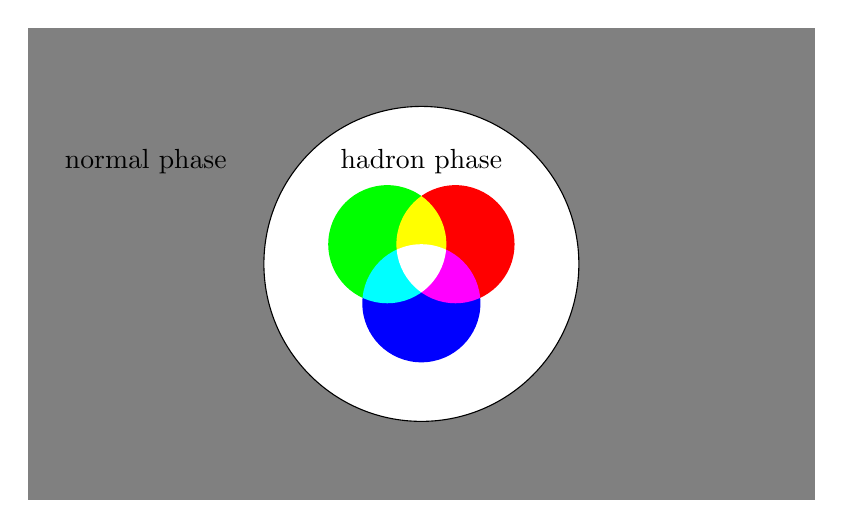
\begin{tikzpicture}
\fill [gray] (-5, -3) rectangle (+5, +3);

\draw [draw=black, fill=white] (0, 0) circle (2);
\begin{scope}[blend group=screen]
	\fill [fill=red]   (30:0.5)  circle (0.75) node {$u$};
	\fill [fill=green] (150:0.5) circle (0.75) node {$d$};
	\fill [fill=blue]  (270:0.5) circle (0.75) node {$s$};
\end{scope}
\node at (90:1.3) {hadron phase};
\node at (-3.5,1.3) {normal phase};
\end{tikzpicture}
\caption{\label{fig:mit:bag_constant}%
	\TODO{finish and try to hammer some ``picture'' into the reader's mind}
}
\end{figure}

A positive bag constant creates a negative vacuum pressure $P = -B$ relative to the \emph{deconfined} phase in the quantum chromodynamics phase diagram in \cref{fig:qcd:phase_diagram},
and can therefore be interpreted as a mechanism that \emph{confines} the quarks to ``bags'' that represent hadrons.
The quarks inside the bag would exert an outwards pressure that counteracts the external bag pressure and stabilizes the bag.
Despite its ad-hoc entry as a mere constant shift of the grand potential,
the bag constant is given the physically vital interpretation as the pressure difference between the confined and deconfined phases
and is an extremely simple way of incorporating confinement in our model.
As an analogy, imagine a swimming pool full of water representing the deconfined phase:
it would cost an amount $BV$ of energy to expel water from a volume $V$ and create a bag of vacuum in the pool,
and a plastic bag covering this volume would have to generate some internal pressure to survive against the pressure from the surrounding water.
The bagging is illustrated in \cref{fig:mit:bag_constant}.

What values can the bag constant take?
Let us perform a heuristic calculation where we picture quarks to be confined in a spherical bag of radius $R$.
The vacuum energy associated with the mere existence of the bag is then $E_V = 4 \pi R^3 B / 3$.
By Heisenberg's uncertainty principle $\Delta p \Delta x \geq \hbar/2$, a quark confined to a region extending $\Delta x = 2R$ in one dimension has momentum $p \gtrsim \hbar/4R$.
In the ultra-relativistic regime where we can neglect mass, the kinetic energy inside the bag is therefore $E_K = pc = C / R$ for some constant $C$.
As a function of $R$, the total energy $E = E_V + E_K$ has a minimum at $R = (C/4 \pi B)^\frac14$ for which the bag is stable.
Solving for $C = 4 \pi B R^4$, the energy of this stable configuration is $E = 16 \pi R^3 B / 3$.
Assuming a neutron with total energy $E = m c^2 = \SI{940}{\giga\electronvolt}$ and radius $R \approx \SI{1}{\femto\meter}$,
the bag constant is
\begin{equation}
	B \approx (\SI{144.4}{\mega\electronvolt})^4 / (\hbar c)^3.
\label{eq:mit:bag_constant_optimal}
\end{equation}

We can use another approach to determine a range of values for the bag constant.
In the early days of the universe with high density and temperature, the universe likely passed through a phase of deconfined quark-gluon plasma.
Today, two-flavor quark matter are accreting in nuclei through fusion towards iron-56 in stars, which seemingly represent the ground state of nuclear matter.
However, \cite{ref:strange_hypothesis_bodmer} and \cite{ref:strange_hypothesis_witten} has hypothesized that this state of matter is only \emph{metastable}
and could decay further to three-flavor quark matter consisting of up, down and strange quarks.
This is referred to as the \textbf{strange matter hypothesis}.
If true, the universe could turn into a very \emph{strange} place some day.

Iron-56 has an energy of $E/N_B = \epsilon/n_B = \SI{930}{\mega\electronvolt}$ per baryon.
If we denote the energy densities of two-flavor and three-flavor quark matter by $\epsilon_2$ and $\epsilon_3$,
then the unstability of two-flavor quark matter and hypothesized stability of three-flavor quark matter at zero pressure $P=0$ imply that
\TODO{at zero pressure}
\begin{equation}
	\frac{\epsilon_3(P=0)}{n_B} < \SI{930}{\mega\electronvolt} < \frac{\epsilon_2(P=0)}{n_B} .
\label{eq:mit:bag_stability}
\end{equation}
This inequality yields a range of acceptable bag constants that we refer to as the \textbf{bag window}.

Let us ultra-relativistic equation of state is affected by the addition of a bag constant
and how inequality \eqref{eq:mit:bag_stability} generates a corresponding bag window.
The bag shift \eqref{eq:mit:bag_shift} changes the equation of state \eqref{eq:mit:eos_ur} to $\epsilon = 3 P + 4 B$.
Neglecting electrons again, the baryon density is $n_B = n_u = \mu_u^3 / \pi^2$,
since $n_d = 2 n_u$ and $n_s=0$ in the two-flavor case and $n_u=n_d=n_s$ in the three-flavor case.
With two flavors we also had $\mu_d = 2^{1/3} \mu_u$,
so the grand potential density \eqref{eq:mit:grand_potential_massless}
yields the pressure $P = (1 + 2^{4/3}) \mu_u^4 / 4 \pi^2 - B$ after ``bagging''.
With three flavors we had $\mu_s = \mu_d = \mu_u$ and instead find $P = 3 \mu_u^4 / 4 \pi^2 - B$.
Setting $P=0$ and eliminating $\mu_u$ in favor of $B$, inequality \eqref{eq:mit:bag_stability} becomes exactly solvable and gives the bag window
\begin{equation}
	%\frac{4 B}{(4 \pi^2 B / 3)^\frac34 / \pi^2} < \SI{930}{\mega\electronvolt} < \frac{4 B}{(4 \pi^2 B / (1+2^\frac43))^\frac34 / \pi^2},
	%\quad \text{or} \quad
	\SI{144.4}{\mega\electronvolt} < B^\frac14 < \SI{162.8}{\mega\electronvolt}.
\label{eq:mit:bag_window_ur}
\end{equation}

Moving back to the general case with nonzero masses,
the program in \TODO{ref appendix} solves inequality \eqref{eq:mit:bag_stability} numerically.
It calculates the baryon density $n_B = (n_u+n_d+n_s)/3$
and performs the shift \eqref{eq:mit:bag_shift} of the pressure and energy density for different bag constants $B$
until it finds the one for which the inequality is barely satisfied.
For the two-flavor and three-flavor equations of state in \cref{fig:mit:eos}, it reports the bounds
\begin{equation}
	\SI{144.3}{\mega\electronvolt} < B^\frac14 < \SI{154.9}{\mega\electronvolt} .
\label{eq:mit:bag_window}
\end{equation}
In all cases, the lower bound comes from the two-flavor case, and the upper bound from the three-flavor case.
Note that the lower bounds in the analytical and numerical bag windows \eqref{eq:mit:bag_window_ur} and \eqref{eq:mit:bag_window}
agree not only with each other, but also with the ``optimal'' bag constant \eqref{eq:mit:bag_constant_optimal}.
In contrast, the upper bounds disagree due to the massless approximation being worse with the addition of the heavy strange quark.

\TODO{for later: get very different $B$ in LSM. but this is because meson potential contributes to effective bag pressure before the crossover?}


\section{Mass-radius solutions}

\begin{figure}[t]%[bh!]
\centering
\tikzsetnextfilename{mit-mass-radius}
\begin{tikzpicture}
\begin{axis}[
	width=15cm, height=12cm,
	xlabel={$R \, / \, \si{\kilo\meter}$}, ylabel={$M \, / \, M_\odot$}, title={Mass-radius diagram for MIT bag-model quark stars}, title style={yshift=2.0cm},
	xmin=0, xmax=15, ymin=0.0, ymax=2.2, xtick distance=1, ytick distance=0.1, minor tick num=9, grid=major,
	point meta=explicit, point meta min=32, point meta max=39,
	colorbar horizontal, colormap name=plasmarev, colorbar style={xlabel=$\log_{10} (P_c \, / \, \si{\pascal})$, xtick distance=1, minor x tick num=9, at={(0.5,1.03)}, anchor=south, xticklabel pos=upper},
	declare function={
		e0 = 4.266500881855304e+37;
	},
	legend pos=north east, legend cell align=right,
]
\tikzset{
	Bpin/.style={gray, sloped, allow upside down=true, rotate=180, yshift=+0.4cm, font=\small},
}
\addplot [black, solid, opacity=0.60] {-1}; \addlegendentry{$N_f=2$};
\addplot [black, solid, opacity=1.00] {-1}; \addlegendentry{$N_f=3$};

% 2-flavor
\addplot+ [solid, mesh, opacity=0.60] table [x=R, y=M, meta expr={log10(\thisrow{P}*e0)}] {../code/data/MIT2F/stars_sigma_800_B14_145.dat}; % node [Bpin, pos=0.920] {$B = (\SI{27}{\mega\electronvolt})^4$};
\addplot+ [solid, mesh, opacity=0.60] table [x=R, y=M, meta expr={log10(\thisrow{P}*e0)}] {../code/data/MIT2F/stars_sigma_800_B14_150.dat}; % node [Bpin, pos=0.920] {$B = (\SI{27}{\mega\electronvolt})^4$};
\addplot+ [solid, mesh, opacity=0.60] table [x=R, y=M, meta expr={log10(\thisrow{P}*e0)}] {../code/data/MIT2F/stars_sigma_800_B14_155.dat}; % node [Bpin, pos=0.920] {$B = (\SI{27}{\mega\electronvolt})^4$};

% 3-flavor
\addplot+ [solid, mesh, opacity=1.00] table [x=R, y=M, meta expr={log10(\thisrow{P}*e0)}] {../code/data/MIT3F/stars_sigma_800_B14_145.dat}; % node [Bpin, pos=0.920] {$B = (\SI{27}{\mega\electronvolt})^4$};
\addplot+ [solid, mesh, opacity=1.00] table [x=R, y=M, meta expr={log10(\thisrow{P}*e0)}] {../code/data/MIT3F/stars_sigma_800_B14_150.dat}; % node [Bpin, pos=0.920] {$B = (\SI{27}{\mega\electronvolt})^4$};
\addplot+ [solid, mesh, opacity=1.00] table [x=R, y=M, meta expr={log10(\thisrow{P}*e0)}] {../code/data/MIT3F/stars_sigma_800_B14_155.dat}; % node [Bpin, pos=0.920] {$B = (\SI{27}{\mega\electronvolt})^4$};
\end{axis}
\end{tikzpicture}
\caption{\label{fig:mit:mass_radius}%
\TODO{add bag constant labels}
Mass-radius solutions of the Tolman-Oppenheimer-Volkoff equation \eqref{eq:master_intro:tov} parametrized by the central pressure $P_c$,
obtained with the two-flavor and three-flavor MIT bag model equations of state from \cref{fig:mit:eos-eos}
modified by the bag shift \eqref{eq:mit:bag_shift} by three bag constants in the bag window \eqref{eq:mit:bag_window}.
}
\end{figure}

Having established the bag window \eqref{eq:mit:bag_window},
different equations of state are finally available to us by ``bagging'' the equation of state in \cref{fig:mit:eos-eos}
with different bag constants inside the window according to the shift \eqref{eq:mit:bag_shift}.
We then solve the Tolman-Oppenheimer-Volkoff equation as described in \cref{sec:master_intro:tov}.
The results are displayed in \cref{fig:mit:mass_radius}.

As we mentioned in \cref{sec:master_intro:tov},
stars with central pressure exceeding that of the maximum mass star are unstable,
so we cut off the mass-radius curve not longer after the peak.
According to the MIT bag model,
quark stars with maximum masses $1.6 \, M_\odot < M < 2.0 \, M_\odot$ and corresponding radii $\SI{9}{\kilo\meter} < R < \SI{11}{\kilo\meter}$ are realizable

Also notice the qualitatively very similar shapes of the mass-radius curves for different bag constants.
In fact, it is possible to show that with the bagged ultra-relativistic equation of state $\epsilon = 3P + 4B$,
the Tolman-Oppenheimer-Volkoff equation \eqref{eq:master_intro:tov} takes on scaling solutions
where the masses $M(B)$ and $M(B')$ and radii $R(B)$ and $R(B')$ corresponding to two different bag constants $B$ and $B'$
are related by $M(B') = \sqrt{B/B'} \, M(B)$ and $R(B') = \sqrt{B/B'} \, R(B)$. \cite[equation 8.29]{ref:glendenning}
These relations hold only approximately in our case, as we have used the massive equation of state.
